
\documentclass[11pt]{article}
\usepackage{amsmath,amssymb,amsfonts} 
\usepackage{epsfig} \usepackage{latexsym,nicefrac,bbm}
\usepackage{xspace}
\usepackage{color,fancybox,graphicx,subfigure,fullpage}
\usepackage[top=1.25in, bottom=1.25in, left=1in, right=1in]{geometry}
\usepackage{tabularx} \usepackage{hyperref} 
\usepackage{pdfsync}
\usepackage[boxruled]{algorithm2e}
\usepackage{multicol}
\usepackage{enumitem}
\newcommand{\parag}[1]{ {\bf \noindent #1}}
\newcommand{\defeq}{\stackrel{\textup{def}}{=}}
\newcommand{\nfrac}{\nicefrac}
\newcommand{\opt}{\mathrm{opt}}
\newcommand{\tO}{\widetilde{O}}
\newcommand{\polylog}{\mathop{\mbox{polylog}}}
\newcommand{\supp}{\mathrm{supp}}
\newcommand{\rank}{\mathrm{rank}}
\newcommand{\ptot}{p_{\mathrm{tot}}}
\newcommand{\pmin}{p_{\mathrm{min}}}
\newcommand{\pmax}{p_{\mathrm{max}}}
\newcommand{\prob}[1]{\mathrm{Pr}\insquare{#1}}


\newcommand{\conv}{\mathrm{conv}}
\newcommand{\dist}{\mathrm{dist}}
\newcommand{\argmin}{\operatornamewithlimits{argmin}}
\newcommand{\sgn}{\mathrm{sgn}}
\newcommand{\fc}{\mathrm{fc}}


\newcommand{\cM}{\mathcal{M}}
\newcommand{\cB}{\mathcal{B}}
\newcommand{\cU}{\mathcal{U}}
\newcommand{\cY}{\mathcal{Y}}
\newcommand{\cF}{\mathcal{F}}
\newcommand{\capa}{\mathrm{Cap}}
\newcommand{\dcapa}{\underline{\mathrm{Cap}}}
\newcommand{\st}{\mathrm{s.t.}}
\newcommand{\un}{\mathrm{un}}

\newcommand{\Pb}{\mathbb{P}}
\newcommand{\sym}{\mathrm{sym}}
\newcommand{\pcount}{\mathbf{PCount}}
\newcommand{\mixdet}{\mathbf{MixDisc}}
\newcommand{\sbold}{\mathbf{S}}
\newcommand{\mb}{{M(\cB)}}

\newcommand{\mlb}{{M_{\mathrm{lin}}(\cB)}}
\newcommand{\redc}[1]{ \textcolor{red} {#1}}
\newcommand{\newt}{\mathrm{Newt}}
\newcommand{\wtf}{\widetilde{f}}
\newcommand{\wt}{\widetilde}
\newcommand{\diam}{\mathrm{diam}}
\newcommand{\lspan}{\mathrm{span}}
\newcommand{\interior}{\mathrm{int}}
\newcommand{\aff}{\mathrm{aff}}
\newcommand{\per}{\mathrm{per}}
\newcommand{\bl}{\mathrm{BL}}
\newcommand{\cE}{\mathbb{E}}


\newcommand{\eps}{\varepsilon}

\newenvironment{proof}{\noindent{\bf Proof:}\hspace*{1em}}{\qed\bigskip}
\clubpenalty=10000
\widowpenalty = 10000
\newcommand{\qed}{\hfill\ensuremath{\square}}


\def\showauthornotes{0} 
\def\showkeys{0} 
\def\showdraftbox{0}


\newcommand{\Snote}{\Authornote{S}}
\newcommand{\Scomment}{\Authorcomment{S}}

\newcommand\Z{\mathbb Z}
\newcommand\N{\mathbb N}
\newcommand\R{\mathbb R}
\newcommand\C{\mathbb C}

\newtheorem{theorem}{Theorem}[section]
\newtheorem{fact}{Fact}[section]
\newtheorem{conjecture}[theorem]{Conjecture}
\newtheorem{definition}{Definition}[section]
\newtheorem{lemma}[theorem]{Lemma}
\newtheorem{remark}[theorem]{Remark}
\newtheorem{proposition}[theorem]{Proposition}
\newtheorem{corollary}{Corollary}[section]
\newtheorem{claim}[theorem]{Claim}

\newtheorem{openprob}[theorem]{Open Problem}
\newtheorem{remk}[theorem]{Remark}
\newtheorem{example}[theorem]{Example}
\newtheorem{apdxlemma}{Lemma}
%\newtheorem{algorithm}[theorem]{Algorithm}
\newcommand{\question}[1]{{\sf [#1]\marginpar{?}} }

%% probability stuff

\newcommand\pr{\mathop{\mbox{\bf Pr}}}
\newcommand\av{\mathop{\mbox{\bf E}}}
\newcommand\var{\mathop{\mbox{\bf Var}}}

\newcommand{\ex}[1]{\av\left[{#1}\right]}
\newcommand{\Ex}[2]{\ap_{{#1}}\left[{#2}\right]}

\def\abs#1{\left| #1 \right|}
\newcommand{\norm}[1]{\ensuremath{\left\lVert #1 \right\rVert}}



\newcommand{\tr}[1]{\mathop{\mbox{Tr}}\left({#1}\right)}
\newcommand{\diag}[1]{{\sf Diag}\left({#1}\right)}

\newcommand\set[1]{\left\{#1\right\}} %usage \set{1,2,3,,}
\newcommand{\poly}{\mathrm{poly}}
\newcommand{\floor}[1]{\left\lfloor\, {#1}\,\right\rfloor}
\newcommand{\ceil}[1]{\left\lceil\, {#1}\,\right\rceil}
\newcommand{\comp}[1]{\overline{#1}}
\newcommand{\pair}[1]{\left\langle{#1}\right\rangle} %for inner product
\newcommand{\smallpair}[1]{\langle{#1}\rangle}

\newcommand{\inparen}[1]{\left(#1\right)}             %\inparen{x+y}  is (x+y)
\newcommand{\inbraces}[1]{\left\{#1\right\}}           %\inbrace{x+y}  is {x+y}
\newcommand{\insquare}[1]{\left[#1\right]}             %\insquare{x+y}  is [x+y]
\newcommand{\inangle}[1]{\left\langle#1\right\rangle} %\inangle{A}    is <A>


\newenvironment{proofsketch}{\begin{trivlist} \item {\bf
Proof Sketch:~~}}
  {\qedsketch\end{trivlist}}

\newenvironment{proofof}[1]{\begin{trivlist} \item {\bf Proof
#1:~~}}
  {\qed\end{trivlist}}


\title{\bf CPSC 464/564: Modeling Alternative Affordable Housing Priority Systems}


\author{Andrew West, Nicole Lam, Atul Pokharel, Urszula Solarz \\
Professor: Nisheeth K. Vishnoi
}





\begin{document}


\maketitle
 
\begin{abstract}
Writing out a detailed model for $N$ individuals and $M$ housing units. 
\end{abstract}
\section{Housing Development Attributes}
Let $M$ be the number of different of housing units. By the Department of Housing and Urban Development, public housing authorities manage a little over $M = $ 1,000,000 units. Each housing unit $m$ is associated with two values: a capacity (number of people who can live in the housing unit) and its vacancy status (1 for occupied, 0 for vacant). Furthermore, we introduce another parameter $v$ that which represents the general vacancy rate (i.e. how many families leave their affordable housing units per period). \\
\newline
Given this list of $M$ housing units, we also want to determine the number of each unique housing type (in terms of size). Namely, we categorize this list of housing units by their capacity $c$. Let us denote the vector of different types of housing by $\mathcal{M}_u$, where each entry of $\mathcal{M}_u$ represents the number of units for each type of house (number of 1 bedrooms, 2 bedrooms, etc.). 
\section{Applicant Attributes}
Let $N$ be the number of applicants to the housing system. Each applicant $1 \leq i \leq N$ has two vectors associated with it: 
\begin{itemize}
    \item A characteristic vector of length $k = 8$, which represents the $k$ different characteristics (family size, income, race, ethnicity, number of children, number of elderly members, veteran status, disability). Below, we describe the parameters we would use if generating synthetic data. Note that we do have existing data from Baltimore that may extend beyond these values.
    \begin{itemize}
        \item Family size - we vary family size between 1 and 8
        \item Income - adjusted gross income of the applicant, we vary between \$1000 and \$100000
        \item Race - categorized by (1) American Indian or Alaska Native, (2) Asian, (3) Black or African American, (4) Native Hawaiian or Other Pacific Islander, (5) White, (6) Multiple Race Combinations
        \item Ethnicity - (1) Hispanic or Latino, (2) Not Hispanic or Latino
        \item Number of children - we vary between 0 and 5
        \item Number of elderly - we vary between 0 and 4
        \item Veteran status - 1 (True) or 0 (False)
        \item Disability - 1 or 0
    \end{itemize}
    Furthermore, in this characteristics table, we add an additional two parameters which we will utilize letter to calculate fairness:
    \begin{itemize}
        \item Wait time - number of periods until the applicant is matched with some housing
        \item Choice number - the ranking of the matched housing unit (i.e. top choice is 1, second choice is 2, ...)
    \end{itemize}
    \item A preference vector $\mathcal{P}_i$ of length $|\mathcal{M}_u|$ that ranks each applicants' preference for each type of housing unit. Recall that each type of housing unit has some capacity $c$. Let us denote the family size of applicant $i$ by $s_i$. \\
    \newline
    We model preferences using the following assumptions: assume that the top preference for every applicant is the housing unit with capacity $s_i$. The next four preferences will include housing units with capacities $s_i \pm 2$. While the top choice does not vary for applicants with the same family size, the next four rankings are ordered at random. Thus, every preference vector $\mathcal{P}_i$ will have an ordering from 1-5, then zero entries at the remaining $|\mathcal{M}_u| - 5$ entries.
\end{itemize} 
\section{Housing Allocation Algorithm}
Consider the following $N$ by $M$ matrix. 
\[H =
\begin{bmatrix}
    \mathcal{P}_1 \\
    \mathcal{P}_2 \\
    \vdots \\
    \mathcal{P}_k
\end{bmatrix}
=
\begin{bmatrix}
    p_{1,1} & p_{1,2} & \cdots & p_{1,M} \\
    p_{2,1} & \ddots & \quad & p_{2,M} \\
    \vdots & \quad & \ddots & \vdots \\
    p_{N,1} & p_{N,2} & \cdots & p_{N,M} 
\end{bmatrix}\]
where $p_{i,j}$ represents the preference ranking for applicant $i$ on housing development $j$. \\
\newline
We introduce two other parameters:
\begin{itemize}
    \item Applicant departure rate $\delta$: at the beginning of each period, we remove $\delta \cdot \texttt{len}(H)$ applicants from the matrix at random. Assume that $\delta$ is constant every period.
    \item Applicant arrival rate $\alpha$: next, we create $X_\alpha \cdot \texttt{len}(H)$ new applicants to add to matrix $H$, where $X_\alpha \sim Poisson(\alpha)$
\end{itemize}
\subsection{Data Set-Up}
\begin{enumerate}
    \item We are given $N$ applicants
    \item Generate a $N \times M$ matrix populated with their preference vectors
    \item Randomly order the rows
\end{enumerate}
\subsection{Initial Run}
Suppose we are allocating housing by some characteristic. For our example, we will use disability.\\
\begin{enumerate}
    \item All housing unit vacancy status is set to 0 (vacant) and set all wait time to be infinite
    \item Remove ineligible applicants (those who's median income is below a certain threshold)
    \item Move all applicants with characteristic \[\texttt{disability[i] = True}\]
    to the top of the matrix.
    \item Iterate through all rows of the matrix
    \item If the top preference of the applicant is vacant, match the housing unit with the applicant and remove the row from the matrix
    \item Set that housing unit's vacancy status to 1, and set that applicant's choice number to be 1
    \item If the top preference of the applicant is not vacant, proceed to the next rankings. Repeat the previous steps (4-5).
    \item If none of the ranked housing units are available, move the applicant to the top of the matrix and proceed to the next iteration.
    \item Add 1 to the wait time of all applicants remaining in matrix $H$.
\end{enumerate}
\subsection{Core Algorithm: Priority Systems}
Continue to suppose we are allocating housing by some characteristic. For our example, we will use disability.\\
\newline
For each period:
\begin{enumerate}
    \item Apply housing vacancy rate $v$, in other words randomly set the vacancy status to be $0$ for
    \[X_v \cdot |M|\]
    housing units.
    where $X_v \sim Poisson(v)$.
    \item Apply applicant departure rate $\delta$. Randomly select $\delta \cdot \texttt{len}(H)$ rows to remove
    \item Apply applicant arrival rate $\alpha$: create $\alpha \cdot \texttt{len}(H)$ new rows and fill with preferences following the same rules described in section 2.
    \item Examine the first row of the matrix
    \item Let us examine the set of plausible housing matches:
    \[J = \{j \mid p_{i,j} > 0\}\]
    \item Choose the column index $j^*$ that that has $p_{i,j^*} = 1$ in $\mathcal{P}_i$.
    \item Examine whether the particular housing unit of size $s_i$ is available:
        \begin{itemize}
        \item If available, match applicant $i$ with housing unit of capacity $s_i$. Set that housing unit as occupied (vacancy status = 1), and mark the choice number of applicant $i$ has 1. Then, remove applicant $i$ from the matrix (remove row $\mathcal{P}_i$)
        \item If not available, proceed to the next ranked housing unit and check for availability. Follow the same rules from the previous step.
        \item If not available and ALL ranked housing units have been checked, move the applicant $i$ to the top of the waitlist and proceed. 
    \end{itemize}
    \item For all applicants $i$ still in matrix $H$, increase their wait time by 1. 
    \item Proceed to the next period. Repeat all steps until matrix $H$ is empty or we have run $10^6$ iterations.
\end{enumerate}
\begin{center}
    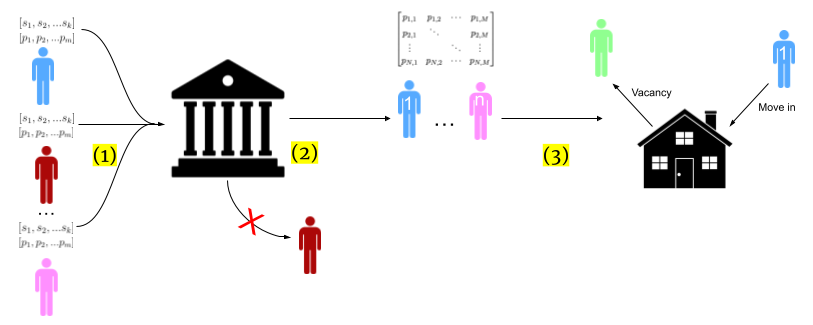
\includegraphics[scale=0.44]{doc/Setup Image.png}
\end{center}
\section{Measurement of Fairness}
We introduce two different measures of fairness.
\subsection{Average Wait Time}
Let $H_1, H_2, \dots, H_\ell$ be subsets of our data, grouped by some characteristic $S_k$. Furthermore, for every applicant $X \in H_k$, let $T_i$ represent the wait time of the applicant $i$ and $t_k$ be the average wait time of applicants in the $k$-th subset. Namely,
\[t_k = \frac{1}{|H_k|}\sum_{i=1}^{|H_k|}T_i\]
Then, we calculate fairness by calculating average wait time for each subset $H_k$, which is organized by characteristic $S_k$. We want $S_k$ and the characteristic used for the priority system to be \text{different}. Then, we measure fairness by the equality group fairness metric:
\[\text{minimize}(t_i - t_j) \quad \text{ for } i \neq j\]
\subsection{Probability of Top Housing Choice}
We introduce another metric of fairness that determines the probability that a certain group gets their top housing choice. \\
\newline
Similarly, let $H_1, H_2, \dots, H_\ell$ be subsets of our data, grouped by some characteristic $S_k$. Recall that each applicant has a characteristic $Y_k$ which tracks their choice number (i.e. whether they got their top choice, second choice, etc.) \\
\newline
Then, we calculate fairness by calculating the probability that an applicant in $H_k$ is matched with their top housing choice. Namely, we measure fairness by aiming to achieve:
\[\frac{P(Y = 1 | H_i)}{P(Y = 1 | H_j)} = 1 \quad \text{ for } i \neq j\]
\section{Desired Results}
We aim to run this algorithm on a few different priority systems, including: high income, low income, disability, veterans status, and number of children. \\
\newline
For each priority system, we will run this algorithm $10^6$ times, calculating the two different metrics of fairness after each simulation. Then, we will plot these two different metrics of fairness and analyze its distribution. \\
\newline
Following that, we will also compare the distribution and statistical summaries of these fairness metrics as we vary different priority systems.
\end{document}
